\chapter{Data Analysis}
\label{ch:data_analysis}
Although we have discussed in detail the theoretical motivations for the W
physics program, as well as the machines producing the necessary collisions and
recording data produced from these collisions, we have not yet addressed the
form of the data set itself, and the substantial engineering it takes to extract
the signal of interest out of that data set.

The relative abundance of the $p + p \rightarrow W^\pm \rightarrow \mu^\pm +
\nu$ signal events is rather low, compared to the other interactions which may
take place when two protons collide. 

The previous chapter how careful triggering is employed in order to ensure that
any time this event does occur, it is recorded. This does not guarantee that
\textit{only} these events are recorded. Background events are still recored
much more frequently than signal events, even with the improved triggering. We
collected 271 $pb^{-1}$ of data (15.7 billion events, according to the PHENIX
run database) from the 2013 dataset, but there are only 3086 $W\rightarrow\mu$
events, after cuts are made (see Chapter~\ref{ch:feature_engineering}).  Of this
subset, assuming a signal to background ratio of 0.2 (this will be motivated and
described in Section~\ref{sec:sbr}), we are left with only 617 `signal events'
out of 15.7 billion total events.

This leads to the substantial problem of extracting the appropriate physics
events from the 15.7 billion event background. 

PHENIX is a multipurpose detector, and has a long history of probing a variety
of physics at a wide range of energy scales. The Muon Arms were originally
designed for the reconstruction of much lower energy charmonium dimuon decays,
and although the forward upgrade has allows us to collect most of the
$W\rightarrow\mu$ events as part of our total dataset, the task of
differentiating very high energy muons from sources of background is
challenging. Without a forward nose-cone calorimeter, or substantially more
steel absorber in place, we must resort to statistical methods to differentiate
between signal events, and background events. This is described in
Chapter~\ref{ch:feature_engineering}

\section{Raw Data to Reconstructed Parameters}

Any time a PHENIX trigger condition is satisfied, all of the information
recorded by the PHENIX spectrometer are read out from temporary on-detector
memory, and fed into a data stream that eventually is archived as a `PHENIX Raw
Data File Format' or PRDFF. 

PRDFF data is hierarchical, first being organized by event-type, and
then organized by packet-type.  There are many event types--`DATAEVENTS'
typically carry the information relevant to a physics analysis, whereas other
event-types carry very important QA information for determining the status of
the RHIC apparatus, the beam, polarization, and PHENIX performance.

Every packet has a header, which contains general information such as what the
packet contains, and in what order that packet was received. Every packet
recorded can be associated with a unique event-sequence number, which specifies
roughly the order in which the event owning the packet was received by the DAQ.
Within a given run number, an event-number is guaranteed to be unique. The
complexity of the packet is limited by the bandwidth available to move data off
PHENIX onto other storage, and the buffers/reconstruction ability of the front
end electronics modules built onto PHENIX subsystems. PHENIX archives data from
the DAQ at a rate of approximately 700 Megabytes per second--or one compact
disk.

Generally, raw PHENIX data is too complex to use straight-away, because minimal
to no reconstruction of physical properties for a certain event is done, due to
hardware limitations and time limitations--some of this raw data is often
directly used in triggering decisions, which must be made once every 106
nanoseconds or faster (the bunch crossing frequency).

The raw data collected from PHENIX undergoes a process called ``Data
Production'', where physical parameters are reconstructed from the simpler raw
data. Raw data could take any form--for example--which cathode strips were
activated in an event in the muon tracker, or, the number of photons counted in
a photomultiplier tube. This information is often combined with extensive survey
information about the geometry of a given detector, the known magnetic field in
a detector, to reconstruct quantities such as momentum, or deposited energy.

Once reconstruction has finished in a Data Production, the data are then
repackaged into ROOT files, often times internally structured into custom output
objects which are associated with a specific detector. These output objects are
simply custom C++ classes which have a serialization scheme, which have
libraries and dictionaries compiled that allow for them to be serialized into
ROOT's file format.

For the purposes of this analysis, all data has been reconstructed and
serialized into a specific type of output object called a `picoDST' or even more
concisely, `pDST'. This name, like many others in PHENIX has historical context:
DST stands for `Data Summary Tape' hearkening back to the days when data was
stored primarily on magnetic tape (it is still archived on magnetic tape!), and
`pico' because of its relatively small disk-space requirement, compared to
`nanoDST' files or simply `DST' files, which contain more granular information.

\section{Choosing Analysis Variables}


Even data reduced to the point of a pDST contains a rich and comprehensive array
of features describing the data--far more than what was ultimately used in this
analysis.  This was largely pragmatic--one can characterize the data streaming
from our detectors in many ways, and detectors themselves can be highly
granular, with each functional piece of a detector producing a stream of data.

Rather than assuming from the outset that we know which variables will provide
the most analyzing power, we observe a variety of data, and perform studies to
determine which combination of variables offers the maximum analyzing power.


The only variables which are truly relevant to this analysis need to be relevant
to understanding two questions:

\begin{enumerate}
  \item \textit{Is this reconstructed muon track the result of a real $W$ Boson Decay?}
  \item \textit{What is the polarization of the two colliding protons for every recorded collision?}
\end{enumerate}

{\noindent}To properly answer these questions, one needs to comprehensively
understand what processes are capable of producing muons, as well as whether or
not our detector can be `tricked' by signals which look like muons, but really
aren't.  Secondly, there must be a means of recovering the proton spin
polarization for each colliding bunch-pair.

The variables used in this analysis are summarized in Tables
\ref{tab:evt_variables},\ref{tab:mutr_variables}, \ref{tab:fvtx_variables} and
\ref{tab:rpc_variables}. When Cartesian coordinates are referenced, implicitly,
the reference frame is the PHENIX Coordinate system
(Figure~\ref{fig:phenix_coordinate_system}).

\subsection{Beam Polarization}

Polarization recovery is relatively straight-forward. Each event is uniquely
mapped to a specific colliding bunch (1,2,...,120). In turn , known `spin
patterns' are applied to each fill, which maps polarization direction to each
bunch. 

As discussed previously (Section~\ref{sec:beam_polarization}), quality assurance
apparatuses are in place to ensure the advertised spin pattern is the same as
that delivered. Since polarization patterns do not typically change in a
standard physics beam fill all that is needed is to associate a PHENIX run
number, with a RHIC fill number, and then look up the spin pattern a database.
If problems were found in the spin pattern during data taking, or later after
scrutiny, the associated data is discarded. The overall beam polarization
percentage is an important factor, which dilutes any spin asymmetry, but this is
taken into account in the final spin database QA analysis~\cite{Kim2014}, the
results of which are summarized in Section~\ref{sec:measured_beam_polarization}.

We are left with the challenging task of differentiating between signal
$W\rightarrow\mu$ events from other $X\rightarrow\mu$ events. This requires that
we engineer features from the data set which are sensitive to the difference
between signal and background. This task is challenging because the
reconstruction characteristics of our detector make it difficult to
differentiate between signal and background without employing sophisticated
statistical models to sort our data set (Section~\ref{sec:likelihood}).


\subsection{Data Analysis}

The thrust of the Data Analysis portion of this work is to separate the real
W-genic muons from all other muon candidates. This requires some substantial
feature engineering, creating statistical models, and a means of evaluating the
performance of these statistical models. Validating our model can be difficult
because since it requires a labeled data set. One way of model validation
employs simulating the entire data set, thus providing every muon track with a
label, and applying the statistical model to this simulated data set. This
analysis was presented in~\cite{Seidl2014a}, lending confidence to our results.

\subsection{Data Analysis--Part 1}

In the first stage of the analysis, the variables used are: DG0, DDG0, DCA$_r$,
$\chi^2$, Rpc1DCA, Rpc3DCA, $fvtx_{dr \times d\theta}$, $fvtx_{d\phi}$, and
$fvtx_{cone}$. These variables are all related to track reconstruction, and were
chosen because they offer the most analyzing power in differentiating between
signal events and background events. Schematically, the variables are described
in Figure~\ref{fig:kinvar_side_view} and \ref{fig:kinvar_beam_view}. These
variables are chosen to be used in the Likelihood Event Selection, which is
described in Section~\ref{sec:likelihood}. Likelihood event selection us used as
an secondary cut on data, after the basic cut, described in
Section~\ref{sec:basic_cut}.

\begin{figure}[ht]
  \centering
  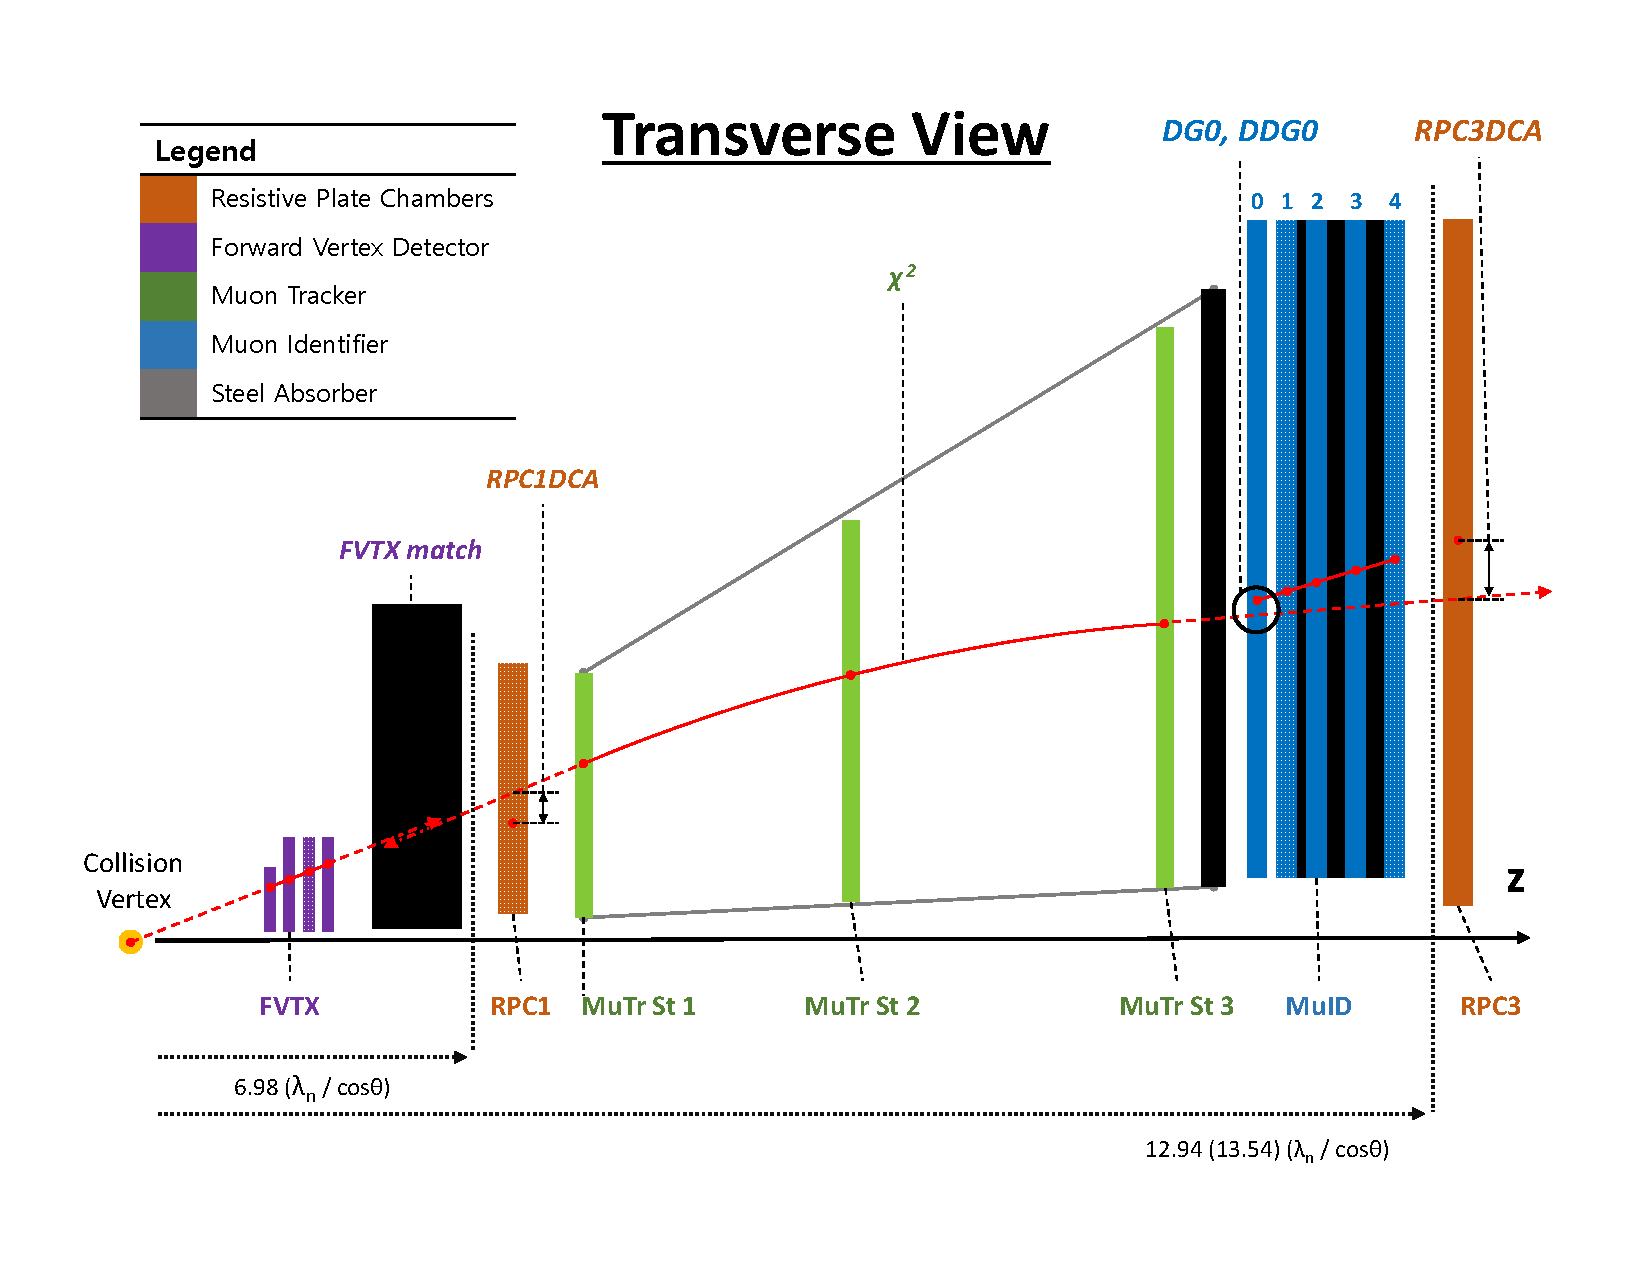
\includegraphics[width=\textwidth]{./figures/kinvar_side_view.pdf}
  \caption{
    Shown: A transverse-view of the FVTX, RPCs, MuTR, and MUID, with
    variables engineered from track reconstruction (track shown as red arc from
    yellow collision point on left)~\cite{Kim2016}
  }
  \label{fig:kinvar_side_view}
\end{figure}
    
\begin{figure}[ht]
  \centering
  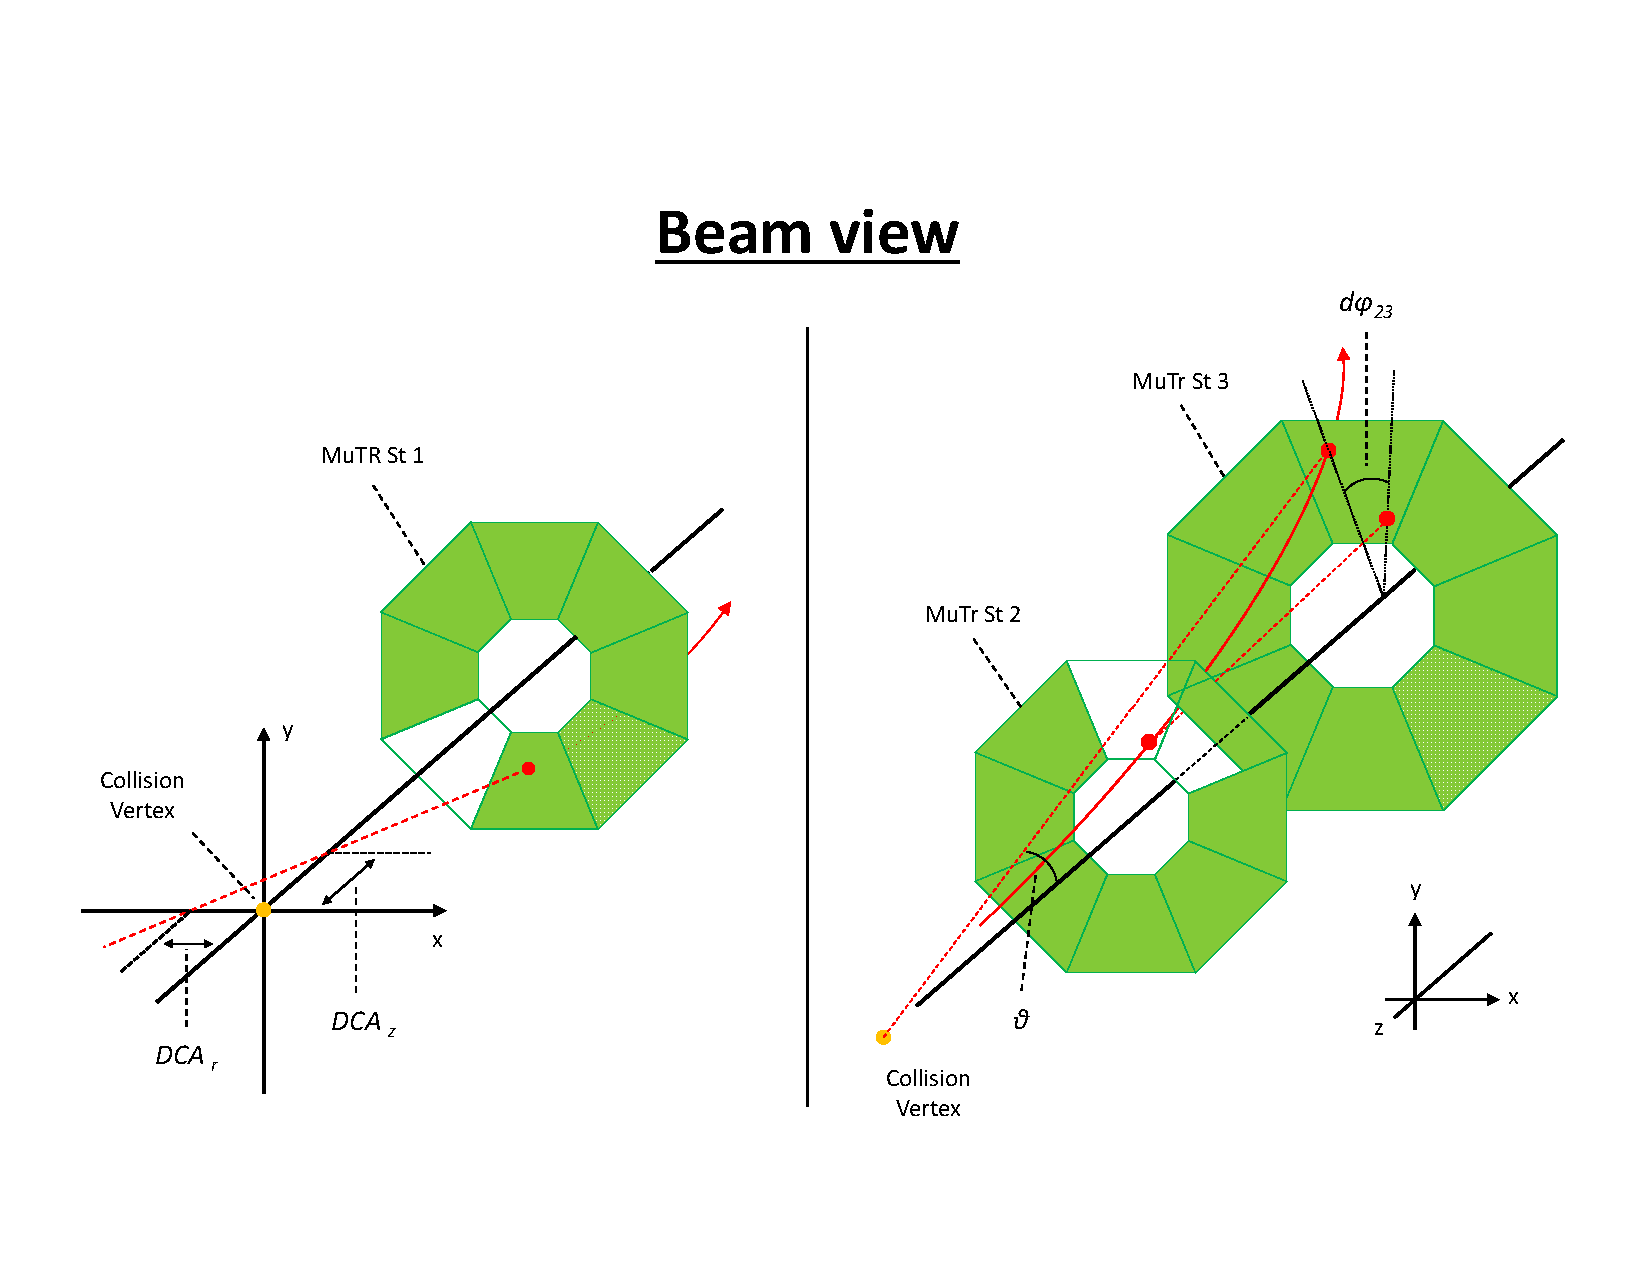
\includegraphics[width=\textwidth]{./figures/kinvar_beam_view.pdf}
  \caption{
    Shown: A beam-view of the MuTR tracking planes with additional variables
    engineered from track reconstruction~\cite{Kim2016}.
  }
  \label{fig:kinvar_beam_view}
\end{figure}

Muon tracks are reconstructed by essentially connecting the dots between `hits'
recorded at each station of the Muon Tracker.  The lines connecting these hits
are called `roads'.  Following this, the roads and hits are used to generate a
curve fit to the data, given knowledge of the muon tracker's radial magnetic
field. This curve, with knowledge of the Muon Trackers' magnetic field, is used
to obtain the charge and momentum of tracks.  Subsequently, variables are
constructed to describe the difference between the reconstructed curve, and the
`connect the dots' roads.  The smaller these differences are, the more straight
the track is, and as discussed, straightness points to higher momentum, which
ultimately leads to labeling as a W-genic particle, if the momentum is in the
correct range.

\subsubsection{DG0 and DDG0}

As seen on the left of Figure~\ref{fig:kinvar_side_view}, DG0 and DDG0
(Figure~\ref{fig:dg0_ddg0_schematic}) are variables defined relative to the
reconstructed muon track, and the road through the MUID. Concretely, the angle
that the reconstructed track makes with the road at station 0 of the MUID
defines DDG0, while the absolute distance between the track and road at MUID
station 0 defines DG0. High momentum tracks, with less bend are correlated with
both of these variables being small. Because DG0 and DDG0 are necessarily
correlated, they require special treatment in the analysis, which is described
fully in Section~\ref{sec:likelihood}.

\begin{figure}[ht]
  \centering
  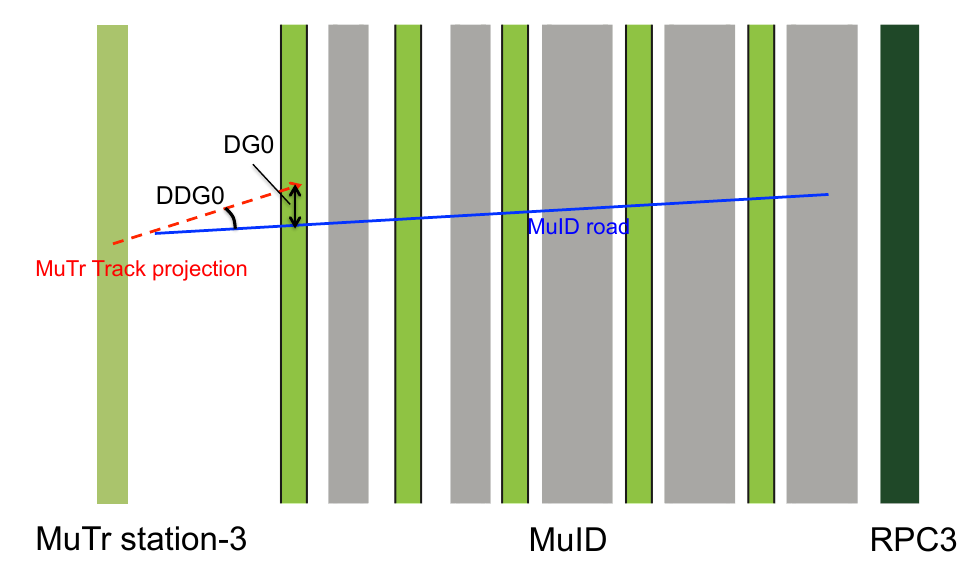
\includegraphics[width=0.7\linewidth]{./figures/dg0_ddg0.png}
  \caption{
    A schematic representation of track-matching variables DG0 and DDG0 at the
    intersection between the Muon Tracker and Muon Identifier~\cite{Oide2012}.
  }
  \label{fig:dg0_ddg0_schematic}
\end{figure}

\subsubsection{DCA$_r$, $\chi^2$, DCA$_z$}

The `distance to closest approach' (DCA$_r$) and `distance of closest approach
z' (DCA$_z$) are shown on the left of Figure~\ref{fig:kinvar_beam_view}. DCA$_r$
is defined to be the distance between the reconstructed track and the beam axis
in the transverse direction, measured at the collision vertex. DCA$_z$ is
defined similarly, except the relative distance interval is between the
collision vertex and the track's z-position at the point where DCA$_r$ is
evaluated. These
distances are useful for evaluating the reconstructed track's probable origin.
The closer to the primary event vertex, the better, as the $W$-Boson is an
interaction associated with the primary event vertex. $\chi^2$ is the reduced
chi-square associated with the quality of track fitting. The chi-square is the
resulting parameter from the Kalman filter based on the `residuals between the
measured coordinate of the cathode planes' of the Muon Tracker after taking into
account position resolution and energy losses~\cite{Oide2012}.

Because DCA$_r$ and $\chi^2$ are correlated, they require special treatment in
the analysis, which is described in Section~\ref{sec:likelihood}.
Grouped for correlation

\subsubsection{RPC Variables}
Rpc1DCA, Rpc3DCA refer to the distance of closest approach at RPC station 1 and
station 3, of the linearly extrapolated track to the closest RPC strip
associated with a hit-cluster on the RPC. These variables are shown at the
position of the RPC1 and RPC3 in Figure~\ref{fig:kinvar_side_view}.

\subsubsection{FVTX Tracking}
The Forward Vertex Detector provides additional tracking information which can
be used to identify events that originate from secondary decays, outside the
primary event vertex. $fvtx_{dr \times d\theta}$ is the product of two FVTX
tracking variables, $fvtx_{dr}$ and $fvtx_{d\theta}$. The product is taken to
reduce the dimensionality of the variable set, because the two quantities are
highly correlated. The FVTX hits are matched to the reconstructed Muon Track,
with $fvtx_{dr}$ representing the residual between the reconstructed FVTX track
and the reconstructed Muon Tracker track in the transverse direction, with
$d\theta$ and $d\phi$ representing the residuals of similar matching in the
canonical $\phi$ and $\theta$ directions. These variables are summarized in
Table~\ref{tab:fvtx_variables}.

\subsubsection{Data Analysis--Part 1, Concluding Remarks}

The tracking variables discussed above all characterize the reconstruction of
muon tracks. These variables were chosen due to their sensitivity to differences
in muon tracks likely resulting from $W$-Boson decays versus other sources. This
is exploited by generating probability distributions associated with each
variable in order to calculate the likelihood of a track originating from a
signal event, or a background event, discussed in Section~\ref{sec:likelihood}.

\subsubsection{Data Analysis--Part 2}
\label{sec:dataset_part_2}

In the second phase of the analysis, $dw_{23}$ and $\eta$ are employed.
$dw_{23}$ is associated with the bending of the reconstructed muon track in the
Muon Tracker volume, and is referred to as ``reduced azimuthal bending''. The
distribution of $\eta$ is expected to have distinct distribution, which differs
based on the track source--$W$-Boson decay, other real muons, and hadronic
decays in the Muon Tracker volume which are reconstructed as muon tracks. Due to
$dw_{23}$ and $\eta$ being both relatively uncorrelated to each-other, as well
as the other variables, one can avoid biasing our statistical models by
effectively over-weighting with correlated variables.

$dw_{13}$, $dw_{23}$ are shown schematically in
Figure~\ref{fig:kinvar_beam_view} and are constructed from $d\phi_{13}$, and
$d\phi{23}$.  $d\phi_{ij}$ is taken as the azimuthal bending of the track
between stations $i$ and $j$. 


\noindent$\phi_{i}$ is calculated from the $x$ and $y$ coordinates of tracks
passing through Station $i$ of the Muon Tracker:

\begin{equation}
  \phi_i = tan^{-1}\left({ySta_i \over xSta_i}\right)
  \label{eq:phi_definition}
\end{equation}

\noindent$dw_{ij}$ is constructed from $d\phi_{ij}$ as follows:

\begin{equation}
  dw_{ij} = p_T \times sin(\theta) \times d\phi_{ij}
  \label{eq:dw23_definition}
\end{equation}

{\noindent}Equation~\ref{eq:dw23_definition} is a proxy for the amount of
bending of a track between stations $i$ and $j$, which is strongly correlated to
the momentum of the track. 

A common theme amongst these variables is that they should help us distinguish
between high momentum muon tracks from $W$ Bosons, and other muon tracks. The
procedure depends on the expectation that W-genic muon tracks are kinematically
restricted to have a relatively narrow momentum distribution. Tracking variables
can be used to partially differentiate between signal and background events.

In general, W-genic events will be mostly straight, geometrically, and so this
constrains the values of variables such as DCA${}_r$ substantially, and other
variables less so. Thus, $dw_{23}$ should be a good discriminator, as it depends
on $p_T$ and the azimuthal bending of the charged tracks, due to the radial
magnetic field in the MuTR.

Our secondary requirement of our variables is that they are relatively
uncorrelated with each-other, to leave plenty of room for statistical modeling.
Ultimately, a subset of the available tracking variables are used to carry out
the analysis, in two stages. The correlation of variables for both data and
simulation are summarized in Figure~\ref{fig:kinematic_var_correlations}.

Since we are interested in recovering forward rapdity $\mu+$ and $\mu-$, and
backward rapidity $\mu+$ and $\mu-$ which result from $W$-Boson decay, we
partition the dataset into these four categories, and perform the analysis on
each category in parallel. 

The data are further subdivided based on the available track matching variables
for a given event. Not all tracking variables are available for every
reconstructed track, because not all detectors have been triggered in the same
way for every event. This is further discussed in the next chapter.

\clearpage
